\chapter{Features}
\section{Users}

The users are the main actors within the application. They share documents, work together and start discussions with each other. Whenever
a user either signs up with a default account, or signs in with a social account, a new user model gets created within the application which then
stores its relations with projects, discussions and files. Every user is connected to a project through a role. The application caters three roles: 
Owner (students), Reviewer (teachers) and Guests (other).

\subsection{Authentication}

Users are able to authenticate themselves in two ways: a default account and through a Google Plus account. A default account can be created from the 
sign up page, where a user is asked for his first and last name, his email address, and his self-chosen password. After the user has submitted his 
information, a verification mail is sent to his email address. An unverified user has no access to the application, so he will be redirected to the 
login page every time as long as he remains unverified. The second type of authentication is through
Google Plus, where a user can identify himself through his Google account. When a user signs in through Google Plus, the application inherits
the first and last name the user has on Google Plus.

\subsection{User roles}

The users of the AssisTU application can be divided into three roles: the owner (students), the reviewer and the guest. The owner role allows for the 
most control over a project. It is the highest ranking role with the least restrictions in terms of actions.
Owners can add or remove members, and (given the role of other participants) sometimes also files and discussions. Besides this, Owners are also 
allowed to edit the name, folder and description of a project of which they are the owner of, regardless of the initial creator. 
The reviewer role is reserved for teachers and supervisors. They get special attention within the application and can easily be visually identified by 
other users. Their contributions into a project in terms of files or comments cannot be deleted by anyone else but themselves, not even by the owners. 
The final role is the guest role. Guests are considered to be neither owners nor reviewers, the guest role is considered the role with the most 
restrictions.

\newpage

\subsection{Mendeley Library Sharing}

During the course of this project, a requirement had been added to allow users to share their Mendeley libraries with other users. A user can
link his mendeley account to the application from the drop down menu on the top right of the application. Once a user has linked his account,
his documents will appear in a mendeley document list within a project, that can only be seen by other mendeley-enabled owners. This list will show
all (distinct) documents from all owners that have linked their mendeley account. The documents that the user already has in his mendeley library
will have a `checked' icon attached to them. The documents that the user does not have in his mendeley library yet will be accompanied by a clickable 
`plus' icon that will push the document to their mendeley library, after which it will also appear as a `checked' icon.

\begin{center}
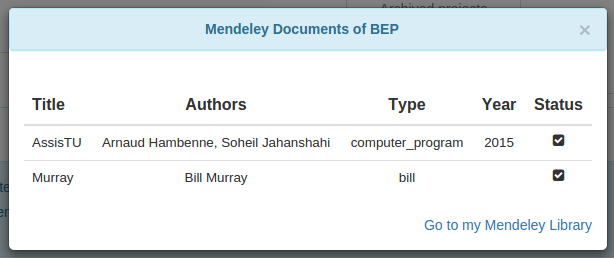
\includegraphics[scale=0.5]{./img/mendeley.png}
\end{center}

\section{Projects}

The main component of the AssisTU application is the creation of, and participation in projects. A project is an entity in which owners, reviewers and 
guests come together. 
The project overview is represented as a series of panels with tables, separated by tabs at the top of the page. The name in the tab is the folder 
name, which is the same name users see when they join the project. 

\subsection{Creating a new Project}

A new project can be created by clicking the `create new project' button on the top left of the project page. When the user clicks this button,
he gets directed to a new page where he can choose a folder name, a project name, a project description and a possible template. The folder name
appears on the tab of both the project- and discussion page, so that users can easily identify which project is under which tab. The project
name is the main name of the project that also appears on top of the discussion page. After the project is created, the user gets redirected
to the project overview with the newest project tab active.

\subsection{Documents}

When a project page is rendered, the user gets to see the list of documents connected to this project. Every member of a project is able to download
any of these documents by clicking the download icon. Only owners and reviewers are able to upload their own documents. When a document is uploaded,
it appears in the list as a row that displays the name of the file, the up-loader, and 2-3 action buttons. The first action button is the download 
button, which is self-explanatory. The second text-balloon-icon action button allows users to use that file as a relational attachment in a discussion.
When they use it, a new page is loaded that displays a new discussion template akin to the one on the discussion page itself. The only difference here
is that now you can see a filename attached to it below the message. The optional third action button is the delete button, which in this case is
only visible if you uploaded the file in the first place. The application does not allow owners to delete files uploaded by other owners or reviewers.

\subsection{Template}

A template is a combination of a file and series of calendar-events. When a user chooses to use a predefined template, he can download the template file
from the project page, and automatically all corresponding events will be loaded inside the calendar view. A user can also choose to create his own 
template if he wishes to. In this case the user can upload his own template file, and create his own events inside the calendar.

\subsection{Project Settings/Options}

After a project is created, the user can see a gear icon in the top right corner of the project panel. Clicking this gear icon shows a drop down
with all the settings and options that a given user (with a given role) is allowed to see.

\begin{center}
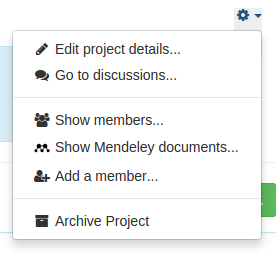
\includegraphics[scale=0.5]{./img/project_dropdown.png}
\end{center}

\subsubsection{Edit Project}

The edit project option is only available to owners. When clicking it, the user get redirected to a page similar to the page where he created a project,
only this time with the data already filled in. The user can either click cancel to cancel the updating of the data, or hit `save'. Note
that a template cannot be re-chosen after the project has been created.

\subsubsection{Go to discussions}

This option is available to all three roles that a user can have in a project. It's basically a direct link to the discussion page of the current
project.

\subsubsection{Show Members}

This option is also available to all three roles. Clicking this option, an overlay screen appears with a table documenting all participating
users, their names, their email addresses, their roles and their status (invited/joined). This is also the screen where owners see a red
delete-icon appear next to certain rows. The rule is that owners cannot remove each other from a project. They can however remove a reviewer 
and a guest, regardless of who invited them originally. Neither reviewers nor guests can remove anyone from a project.

\subsubsection{View Mendeley Library}

Viewing the Mendeley Library is exclusively accessible for owners that have linked their Mendeley account with the application. Clicking this
option renders a list of all documents of all Mendeley-enabled owners within the project. When you already have a listed document in your library, a 
`checked' icon will appear as its status. Documents you do not yet have in your Mendeley Library will appear with a `plus' icon as their status,
which can then be clicked by the user to automatically add the document to their Mendeley Library.

\subsubsection{Invite a Member}

Inviting a member is also an option only available to users who have the owner role within a project. When clicking this option, an overlay
screen appears that has text input for an email address, and a drop down menu where a role can be specified. A valid email address is needed
to invite someone, if you try to invite someone with an invalid email address, nothing happens. An invitation cannot be canceled, the 
invited user must first either accept or decline an invitation.

\subsubsection{Leave Project}

The final option in the drop down menu is the option to leave the project. When clicked, a confirmation overlay screen appears asking the user
if he is sure he wants to leave the project. When accepted, his role gets deleted and he will no longer be able to see the project, or
access any of its files, not even the files he uploaded to it. 

\subsubsection{Archive Project}

A project must always have at least one owner to control it. Therefore the last owner of a project is not able to leave the project, but only
archive it. Archiving a project will remove it from your view, and add it to the table that appears after the user clicks on `archived projects'.

\subsection{Receiving an invitation}

When a user gets invited to a project, the number on the button labeled `invitations' will increment per invitation. This button triggers a drop down
that lists all of the pending invitations. An invitation displays a small text describing the name of the project, and the role as which the user is invited to participate. Below this information are two buttons, the red button declines the request, the green one accepts it.
Note that for design purposes, an icon related to his role is displayed in the front of the invitation block. 
As long as a user does not either accept or decline his invitation, he cannot be invited again for the same project.

\begin{center}
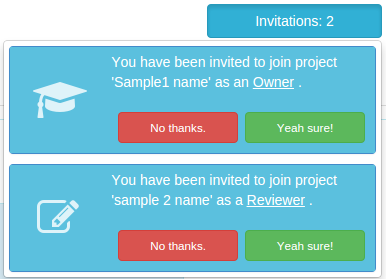
\includegraphics[scale=0.5]{./img/invitation.png}
\end{center}

\section{Calendar}

The calendar is where users can see the planning of all the projects of which they are an owner.
When a predefined template has been chosen, the events on the calendar will already be loaded after
a user has either created or joined a project as an owner. The calendar itself is personal, so users can also add their own events aside from their 
project events. When no predefined template was chosen, you can either
create your own template with personalized events, or have no template and do whatever you like.

\subsection{Creating an Event}

A user can create an event by either clicking on a day in the calendar, or by selecting multiple days by dragging their mouse pointer over these days
as he keeps the mouse button down. When the user releases his mouse button, a browser window appears prompting the user for a name for the event. After
the user has given in a name, a description is also needed. When all the information is provided, and the user clicks on `ok', the event will appear
in the form of a bar through all the days that were selected.

\subsection{Updating Events}

The data of an event, such as name and description can be updated by simply clicking the event in the calendar view. When clicked, an edit event 
form page appears with all the information about the event. Here the user can update the values and click save. It is also possible for users
to update events by simply clicking and dragging them across the calendar screen itself, or by selecting the edges and making them larger or
smaller. Whenever a user performs either of these actions, the start and end dates of the events are automatically updated in the database.
\newpage
\section{Discussions}

The discussions page is a place where all members of a project are free to discuss things with each other. It works the same way a chat would, where
each incoming message immediately appears on another user's screen, only it looks a bit more advanced than just having messages pop up.
The discussion page shares the same top row of tabs as seen in the project view. Clicking one of these tabs
triggers the discussion overview to load for that specific project. In this overview, users gets a
list of subjects, along with the name of the original poster and an icon declaring his role within the project. 
By default all discussions are collapsed. Users can click the `show/hide' button on a specific discussion to 
expand a discussion, which unveils its content and reactions (also called sub-comments).

\subsection{Leaving a comment or reaction}

The user can start a new discussion by clicking the `start new discussion' button. A drop down then appears with a visual template of how the message will appear in the list below after submission.  
Only when a discussion is expanded, an input field appears at the bottom which allows users to leave a reaction to this discussion. 
A reaction left on a message becomes instantly visible to other users who are browsing the same discussion without the need to reload the page to simulate direct conversation.

\subsection{Attaching a file to a comment}

When a file gets uploaded to a project, a small text field icon appears next to that users can click to start
a new discussion with that file attached. This brings them to a separate page where the same template appears
as from the `start new discussion' drop down. The only difference between this feature and the one above is that now an attachment appears at the end of the discussion. 
When submitted the user is taken to the discussion page where the attachment can be visually spotted underneath the subject from a collapsed message.

\section{Tasks}

The tasks page is where the user can create his own personal `todo' list. The view consists of two
panels next to each other where the left one contains tasks that the user still has to do,
and the right panel lists all the tasks that the user has already completed. A user can create
a new task by clicking on the green button with the plus-sign in the top left corner of the `todo' task
panel. An input field appears inside the panel with a calendar icon. When the user has filled out
the task description, and has chosen a deadline on the calendar, he can click on the save button to have
it appear in the list of `todo' tasks. This task object comes with an empty `check off' square on the left,
and the option to delete the task on the right. When the task is done, a user can cross it off his list by
clicking the check-off square in front of the task object. The task then appears crossed of on the panel on
the right where the user can choose to either redo the task, or remove it. Tasks do not appear in the calendar
view as per requirement by the client.

\section{Suggestions}

The suggestion page is not implemented in this version of the application, this version is meant to provide feedback to the creators
to determine how the suggestions should be built in the future. The main idea behind this page is to be able to guide users in their
process of writing a scientific paper or article. Suggestions should be both project-specific and user-specific, which was beyond
the scope of this project at this time.